% Options for packages loaded elsewhere
\PassOptionsToPackage{unicode}{hyperref}
\PassOptionsToPackage{hyphens}{url}
%
\documentclass[
  ignorenonframetext,
]{beamer}
\usepackage{pgfpages}
\setbeamertemplate{caption}[numbered]
\setbeamertemplate{caption label separator}{: }
\setbeamercolor{caption name}{fg=normal text.fg}
\beamertemplatenavigationsymbolsempty
% Prevent slide breaks in the middle of a paragraph
\widowpenalties 1 10000
\raggedbottom
\setbeamertemplate{part page}{
  \centering
  \begin{beamercolorbox}[sep=16pt,center]{part title}
    \usebeamerfont{part title}\insertpart\par
  \end{beamercolorbox}
}
\setbeamertemplate{section page}{
  \centering
  \begin{beamercolorbox}[sep=12pt,center]{part title}
    \usebeamerfont{section title}\insertsection\par
  \end{beamercolorbox}
}
\setbeamertemplate{subsection page}{
  \centering
  \begin{beamercolorbox}[sep=8pt,center]{part title}
    \usebeamerfont{subsection title}\insertsubsection\par
  \end{beamercolorbox}
}
\AtBeginPart{
  \frame{\partpage}
}
\AtBeginSection{
  \ifbibliography
  \else
    \frame{\sectionpage}
  \fi
}
\AtBeginSubsection{
  \frame{\subsectionpage}
}
\usepackage{amsmath,amssymb}
\usepackage{iftex}
\ifPDFTeX
  \usepackage[T1]{fontenc}
  \usepackage[utf8]{inputenc}
  \usepackage{textcomp} % provide euro and other symbols
\else % if luatex or xetex
  \usepackage{unicode-math} % this also loads fontspec
  \defaultfontfeatures{Scale=MatchLowercase}
  \defaultfontfeatures[\rmfamily]{Ligatures=TeX,Scale=1}
\fi
\usepackage{lmodern}
\ifPDFTeX\else
  % xetex/luatex font selection
\fi
% Use upquote if available, for straight quotes in verbatim environments
\IfFileExists{upquote.sty}{\usepackage{upquote}}{}
\IfFileExists{microtype.sty}{% use microtype if available
  \usepackage[]{microtype}
  \UseMicrotypeSet[protrusion]{basicmath} % disable protrusion for tt fonts
}{}
\makeatletter
\@ifundefined{KOMAClassName}{% if non-KOMA class
  \IfFileExists{parskip.sty}{%
    \usepackage{parskip}
  }{% else
    \setlength{\parindent}{0pt}
    \setlength{\parskip}{6pt plus 2pt minus 1pt}}
}{% if KOMA class
  \KOMAoptions{parskip=half}}
\makeatother
\usepackage{xcolor}
\newif\ifbibliography
\setlength{\emergencystretch}{3em} % prevent overfull lines
\providecommand{\tightlist}{%
  \setlength{\itemsep}{0pt}\setlength{\parskip}{0pt}}
\setcounter{secnumdepth}{-\maxdimen} % remove section numbering
\setbeamertemplate{footline}[frame number]
\ifLuaTeX
  \usepackage{selnolig}  % disable illegal ligatures
\fi
\IfFileExists{bookmark.sty}{\usepackage{bookmark}}{\usepackage{hyperref}}
\IfFileExists{xurl.sty}{\usepackage{xurl}}{} % add URL line breaks if available
\urlstyle{same}
\hypersetup{
  pdftitle={Example plots - village profile},
  pdfauthor={Nicholus},
  hidelinks,
  pdfcreator={LaTeX via pandoc}}

\title{Example plots - village profile}
\author{Nicholus}
\date{2024-01-23}

\begin{document}
\frame{\titlepage}

\begin{frame}{Village Characteristics}
\protect\hypertarget{village-characteristics}{}
\begin{itemize}
\tightlist
\item
  \protect\hyperlink{pop}{Population}
\item
  \protect\hyperlink{hfc}{Health facilities}
\item
  \protect\hyperlink{equiptment}{Medicines and Equiptment Supply}
\item
  \protect\hyperlink{healthconcern}{Main health concern}
\item
  \protect\hyperlink{covid}{Covid-19 cases}
\item
  \protect\hyperlink{malnut}{Treated malnourished cases}
\item
  \protect\hyperlink{markets}{Market information}
\item
  \protect\hyperlink{foodprices}{Food commodity prices}
\item
  \protect\hyperlink{vthccsi}{Coping strategies}
\item
  \protect\hyperlink{telecon}{Telecom availability}
\end{itemize}
\end{frame}

\begin{frame}{Village Population (overall sample)}
\protect\hypertarget{pop}{}
\begin{figure}
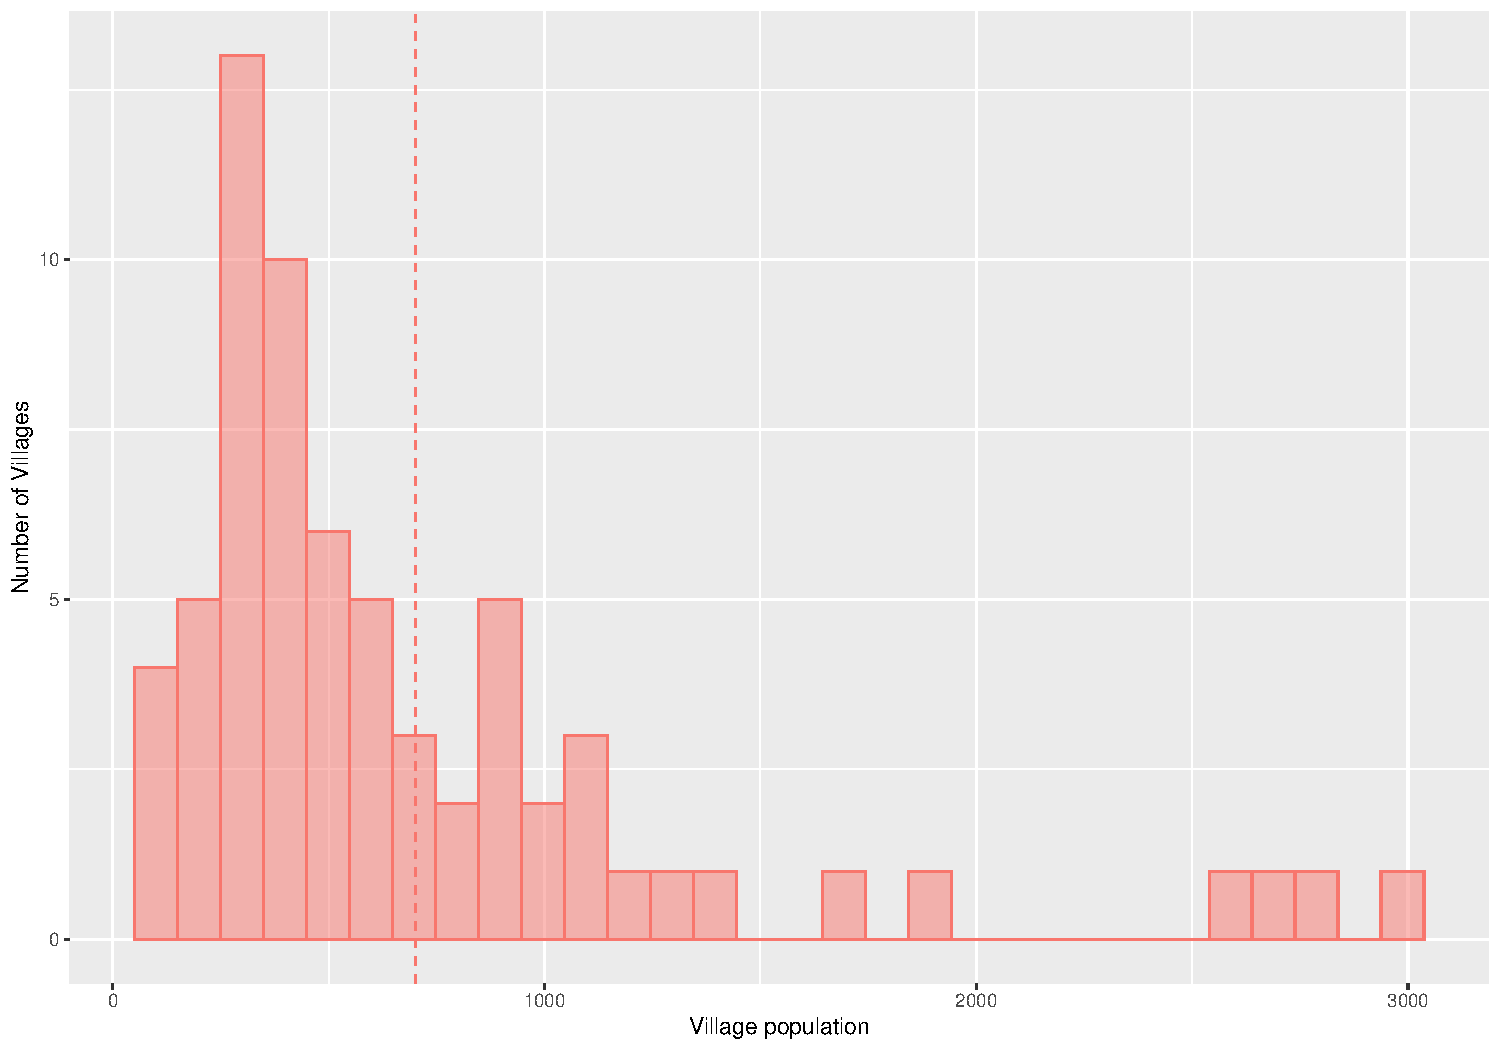
\includegraphics[width=1\linewidth]{example_plots_files/figure-beamer/unnamed-chunk-2-1} \caption{Village population distribution}\label{fig:unnamed-chunk-2}
\end{figure}
\end{frame}

\begin{frame}{Village Population (by sample type)}
\protect\hypertarget{village-population-by-sample-type}{}
\begin{figure}
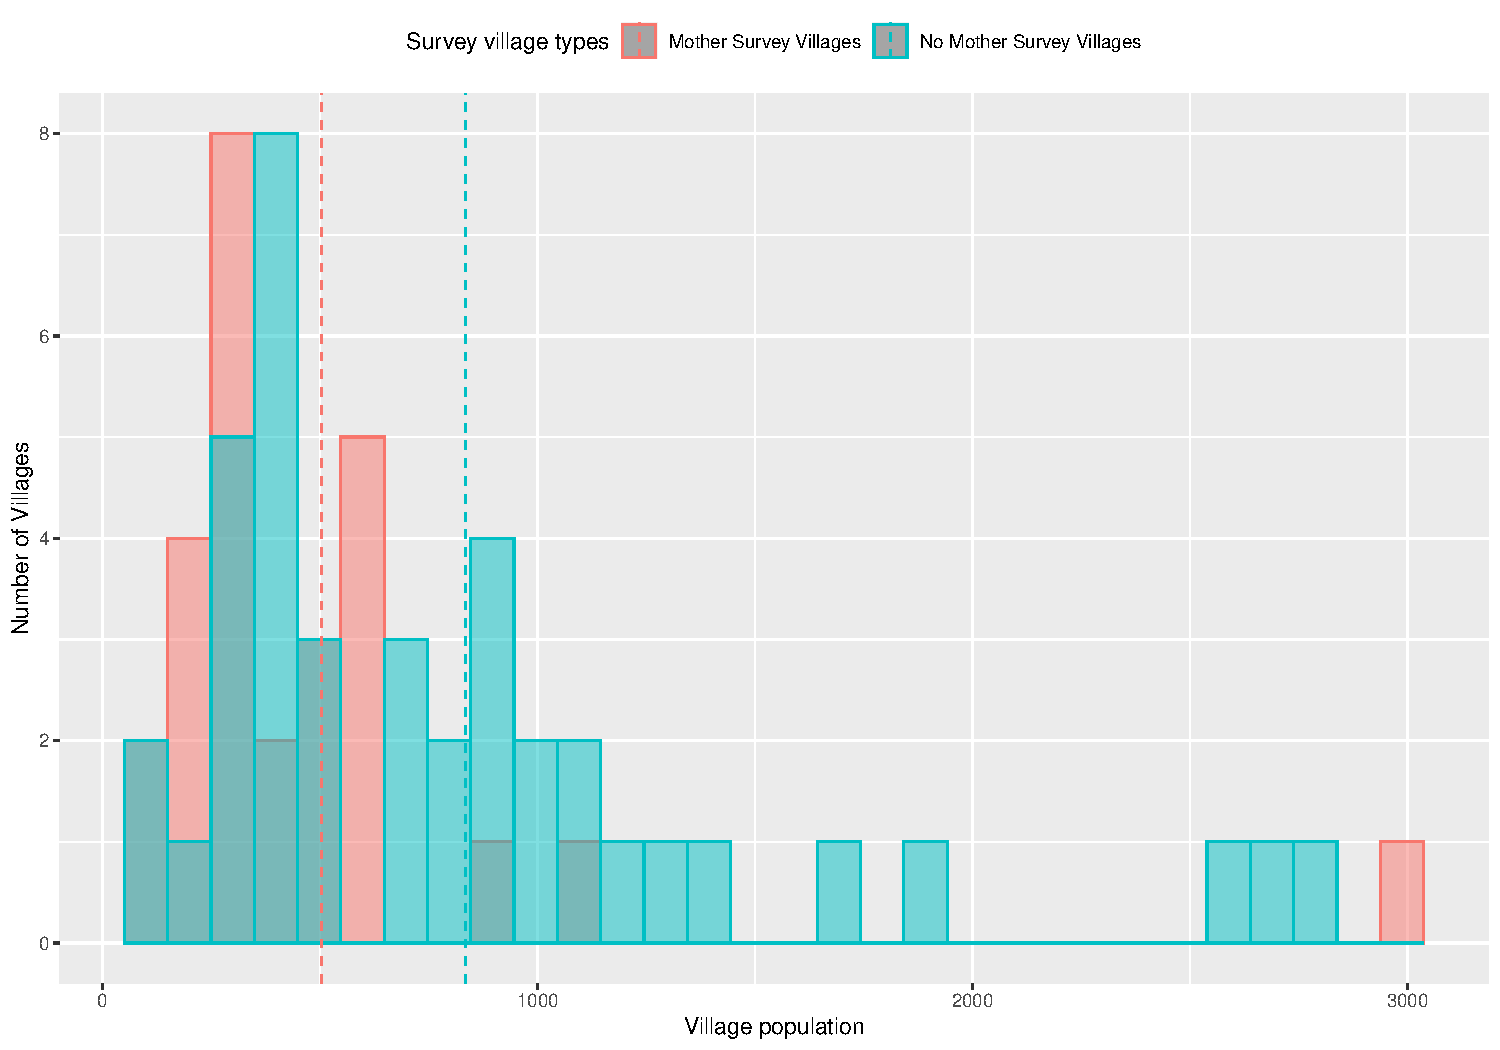
\includegraphics[width=1\linewidth]{example_plots_files/figure-beamer/unnamed-chunk-3-1} \caption{Village Population Distribution per sample type}\label{fig:unnamed-chunk-3}
\end{figure}
\end{frame}

\begin{frame}{Village Population}
\protect\hypertarget{village-population}{}
\begin{itemize}
\tightlist
\item
  wider variation in village population with some outlier villages.
\item
  villages where only VTHC surveys were collected, had higher population
  sizes.
\end{itemize}
\end{frame}

\begin{frame}{Health Facilities (overall sample)}
\protect\hypertarget{hfc}{}
\begin{figure}
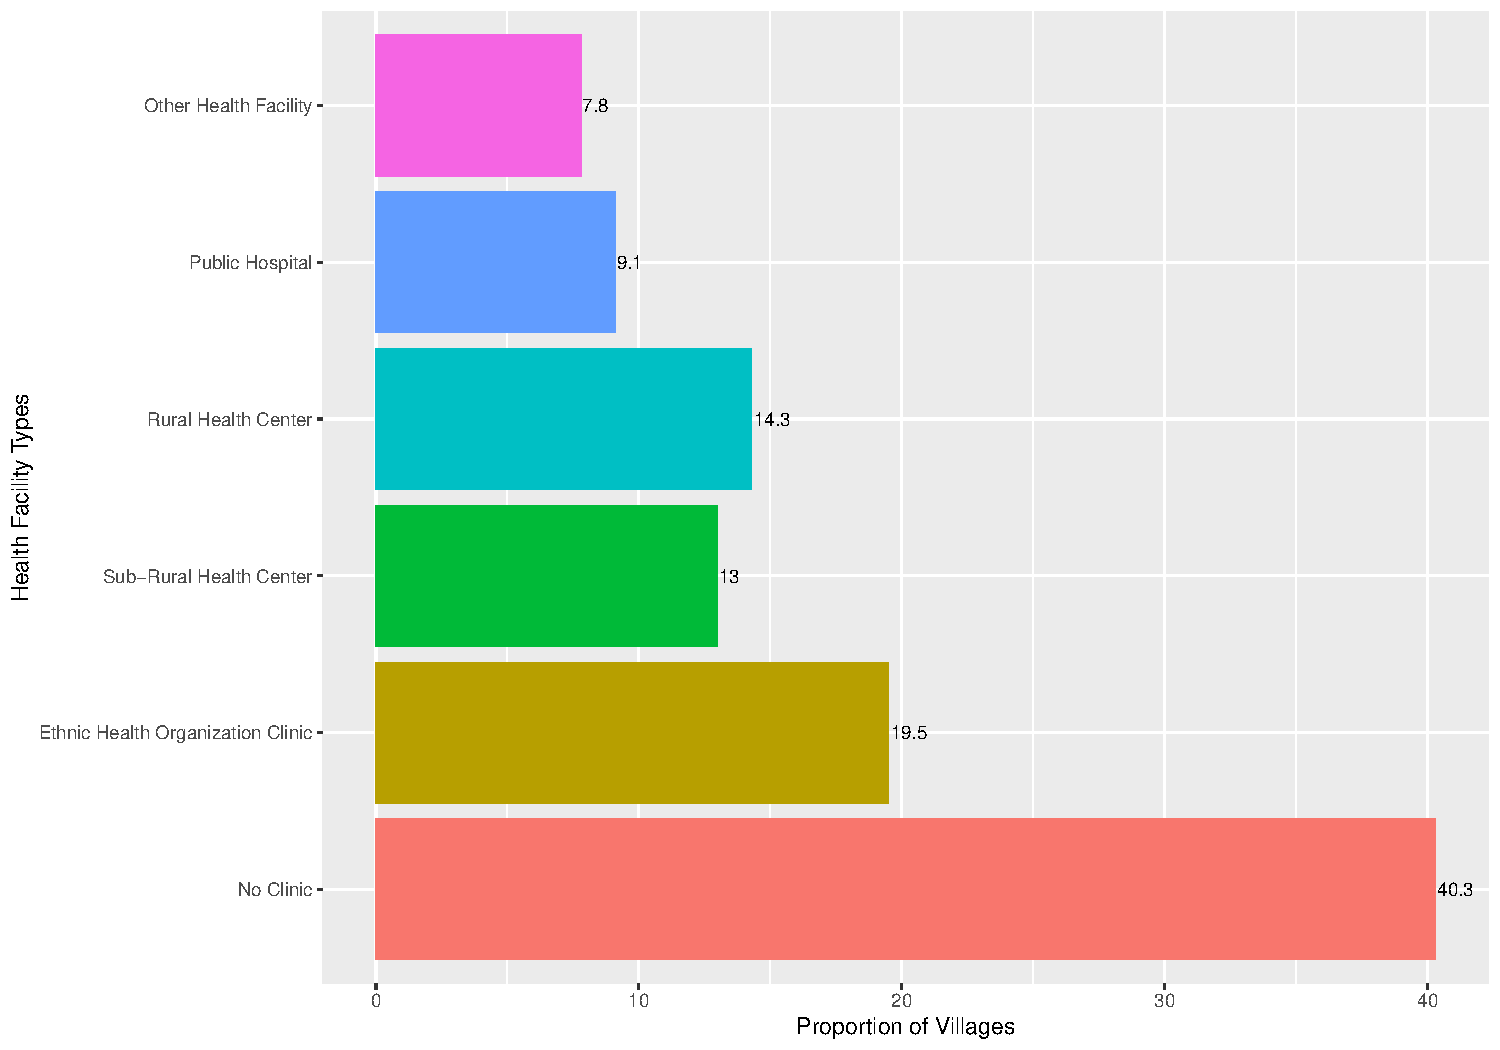
\includegraphics[width=1\linewidth]{example_plots_files/figure-beamer/unnamed-chunk-4-1} \caption{Functioning health facilities (in Village Tract) distribution}\label{fig:unnamed-chunk-4}
\end{figure}
\end{frame}

\begin{frame}{Health Facilities}
\protect\hypertarget{health-facilities}{}
\begin{itemize}
\tightlist
\item
  almost half of the sample (40.3\%) did not have access to the
  functioning clinic(s)
\item
  among the accessible villages, EHO's clinics (19.5\%) shared the
  largest proportion (by individual health facility type)
\item
  but if we combined all the Government health facilities, its share was
  higher than EHO's clinics
\end{itemize}
\end{frame}

\begin{frame}{Medicines and Equipment Supplies (overall sample)}
\protect\hypertarget{equiptment}{}
\begin{figure}
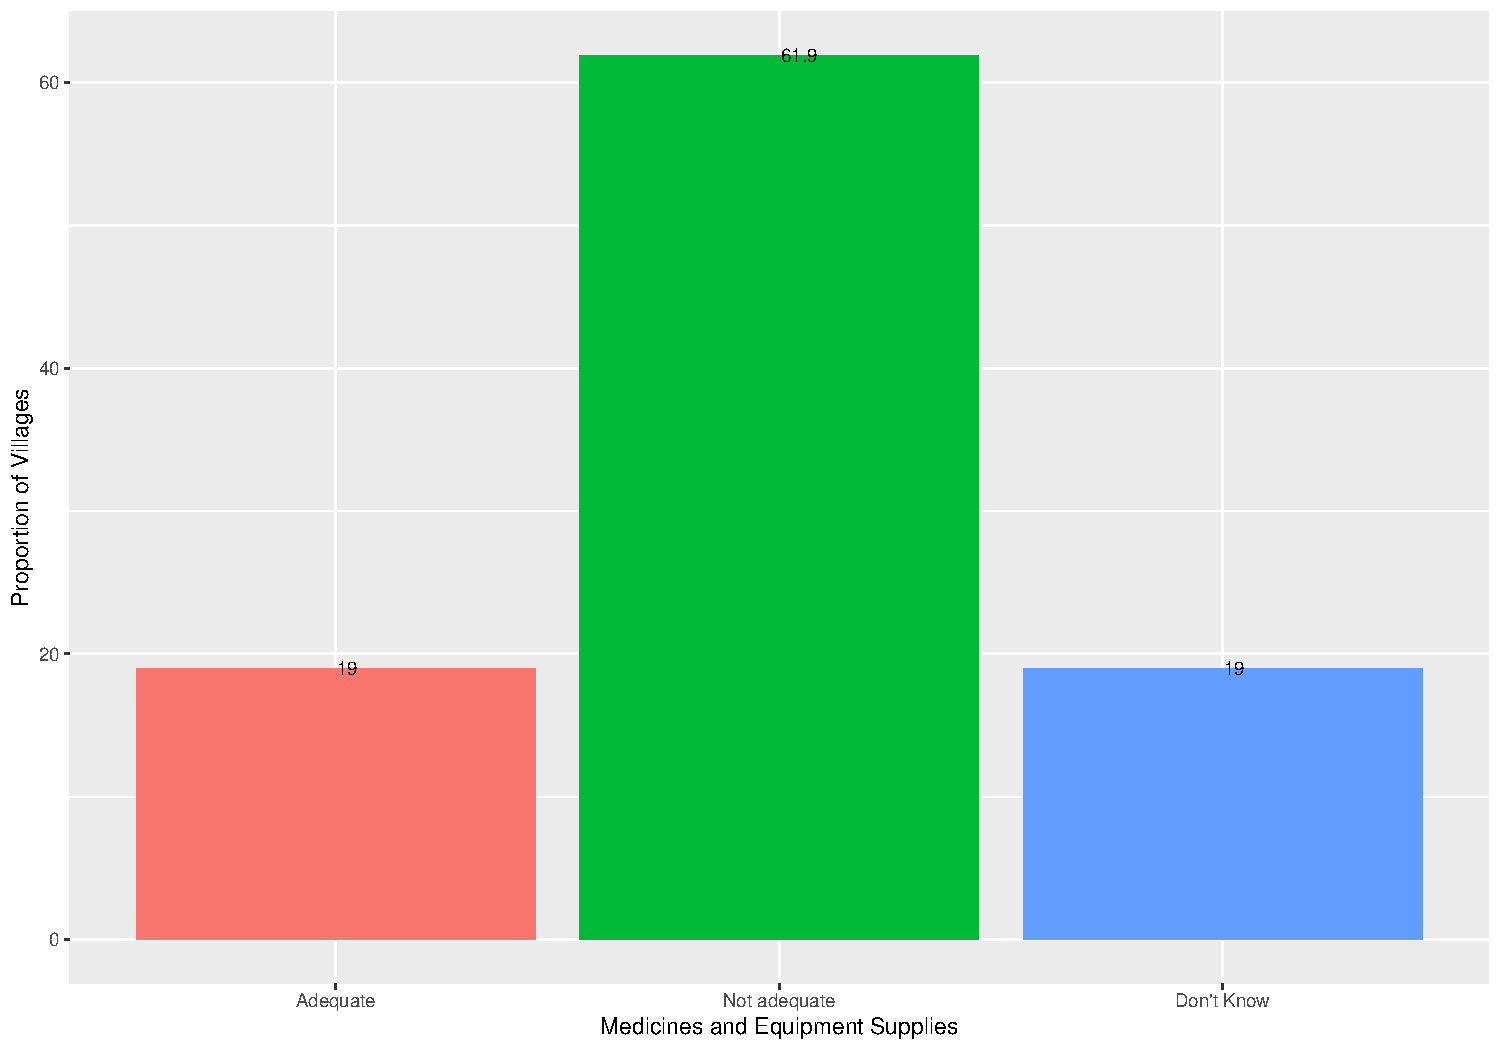
\includegraphics[width=1\linewidth]{example_plots_files/figure-beamer/unnamed-chunk-5-1} \caption{Adequacy of medicines and equiptment supplires distribution}\label{fig:unnamed-chunk-5}
\end{figure}
\end{frame}

\begin{frame}{Main Health Concern (overall sample)}
\protect\hypertarget{healthconcern}{}
\begin{figure}
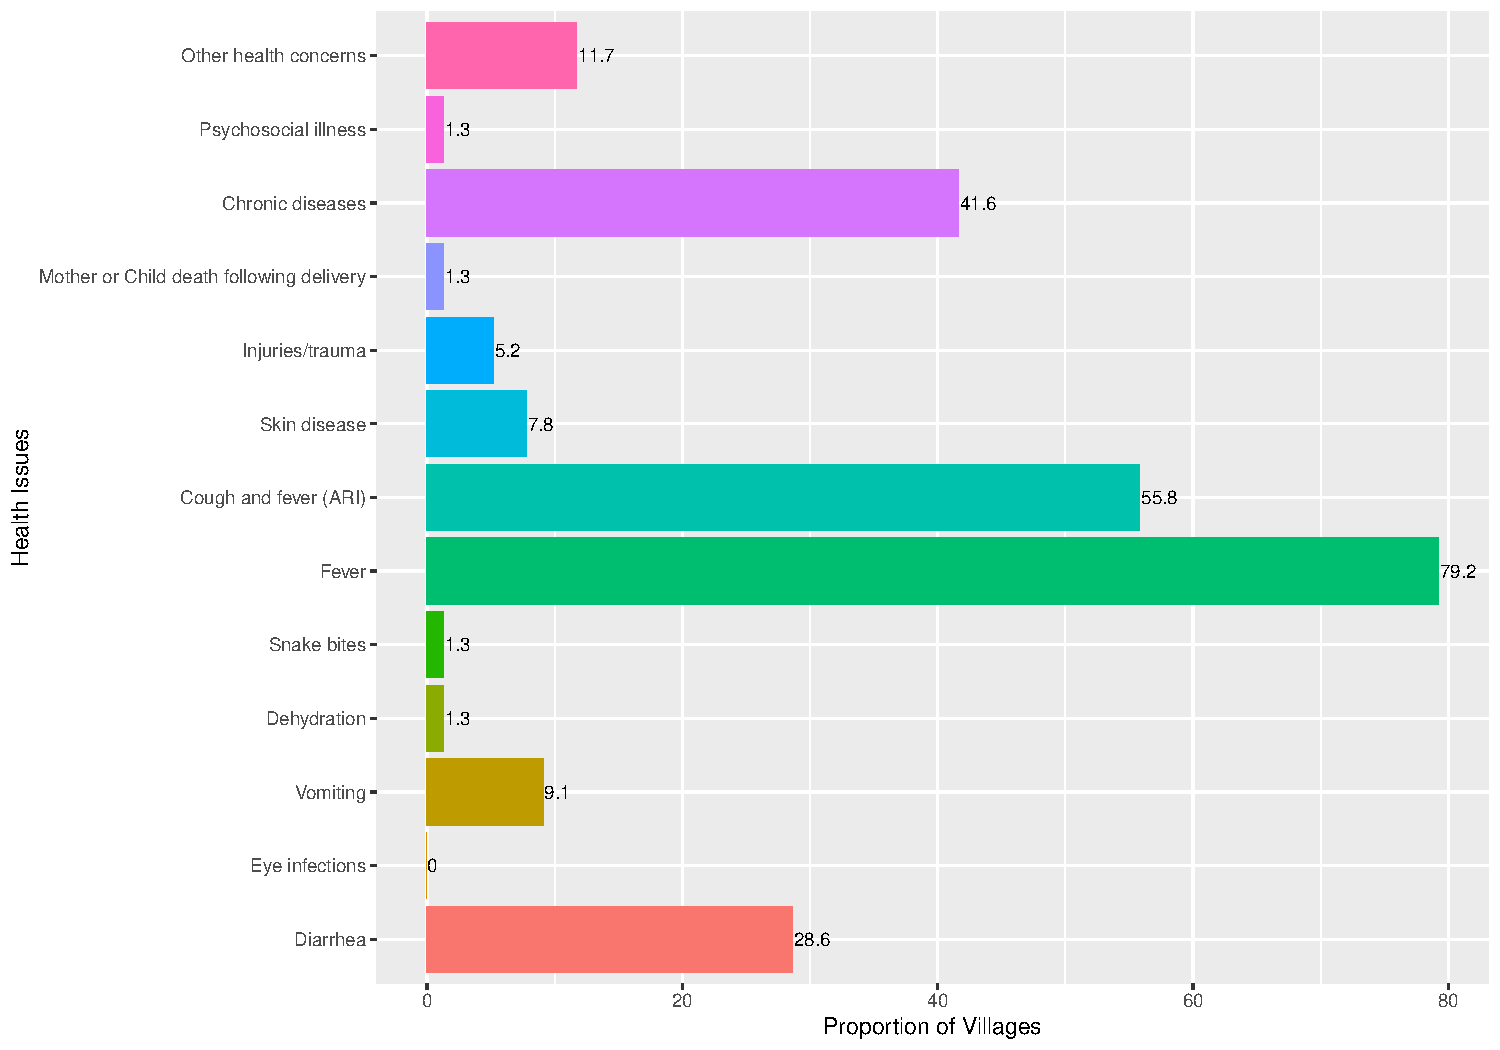
\includegraphics[width=1\linewidth]{example_plots_files/figure-beamer/unnamed-chunk-6-1} \caption{Village main health concern as reported by VHTC}\label{fig:unnamed-chunk-6}
\end{figure}
\end{frame}

\begin{frame}{Main Health Concern (by sample type)}
\protect\hypertarget{main-health-concern-by-sample-type}{}
\begin{figure}
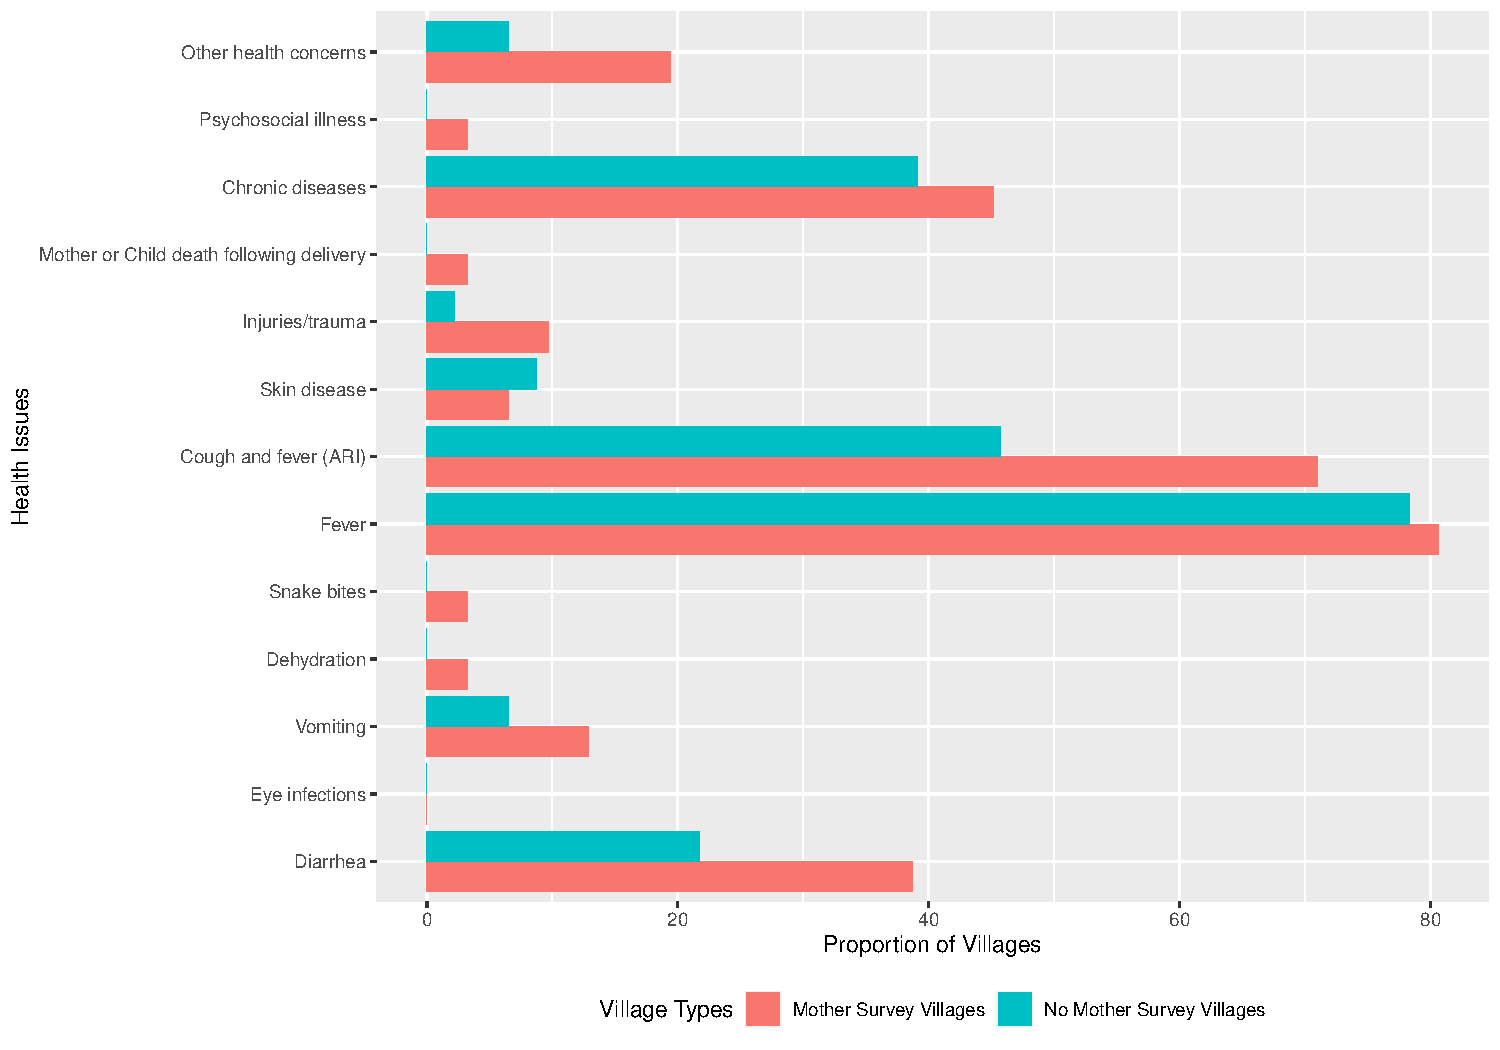
\includegraphics[width=1\linewidth]{example_plots_files/figure-beamer/unnamed-chunk-7-1} \caption{Village main health concern by sample type (as reported by VHTC)}\label{fig:unnamed-chunk-7}
\end{figure}
\end{frame}

\begin{frame}{Main Health Concern}
\protect\hypertarget{main-health-concern}{}
\begin{itemize}
\tightlist
\item
  common childhood illnesses like fever (79.2\%) and cough (ARI)
  (55.8\%) were the most reported diseases\\
\item
  almost half of the village reported non-communicable disease(s)
  (41.6\%)\\
\item
  although the proportion was not higher than other common childhood
  illnesses, diarrhea was reported in a noticeable amount (around one
  out of three - 28.6\%)\\
\item
  mother survey (only) villages had a higher proportion of
  above-reported diseases, and among them, cough (ARI) was statistically
  significant
\end{itemize}
\end{frame}

\begin{frame}{Covid-19 Suspected Cases}
\protect\hypertarget{covid}{}
\begin{figure}
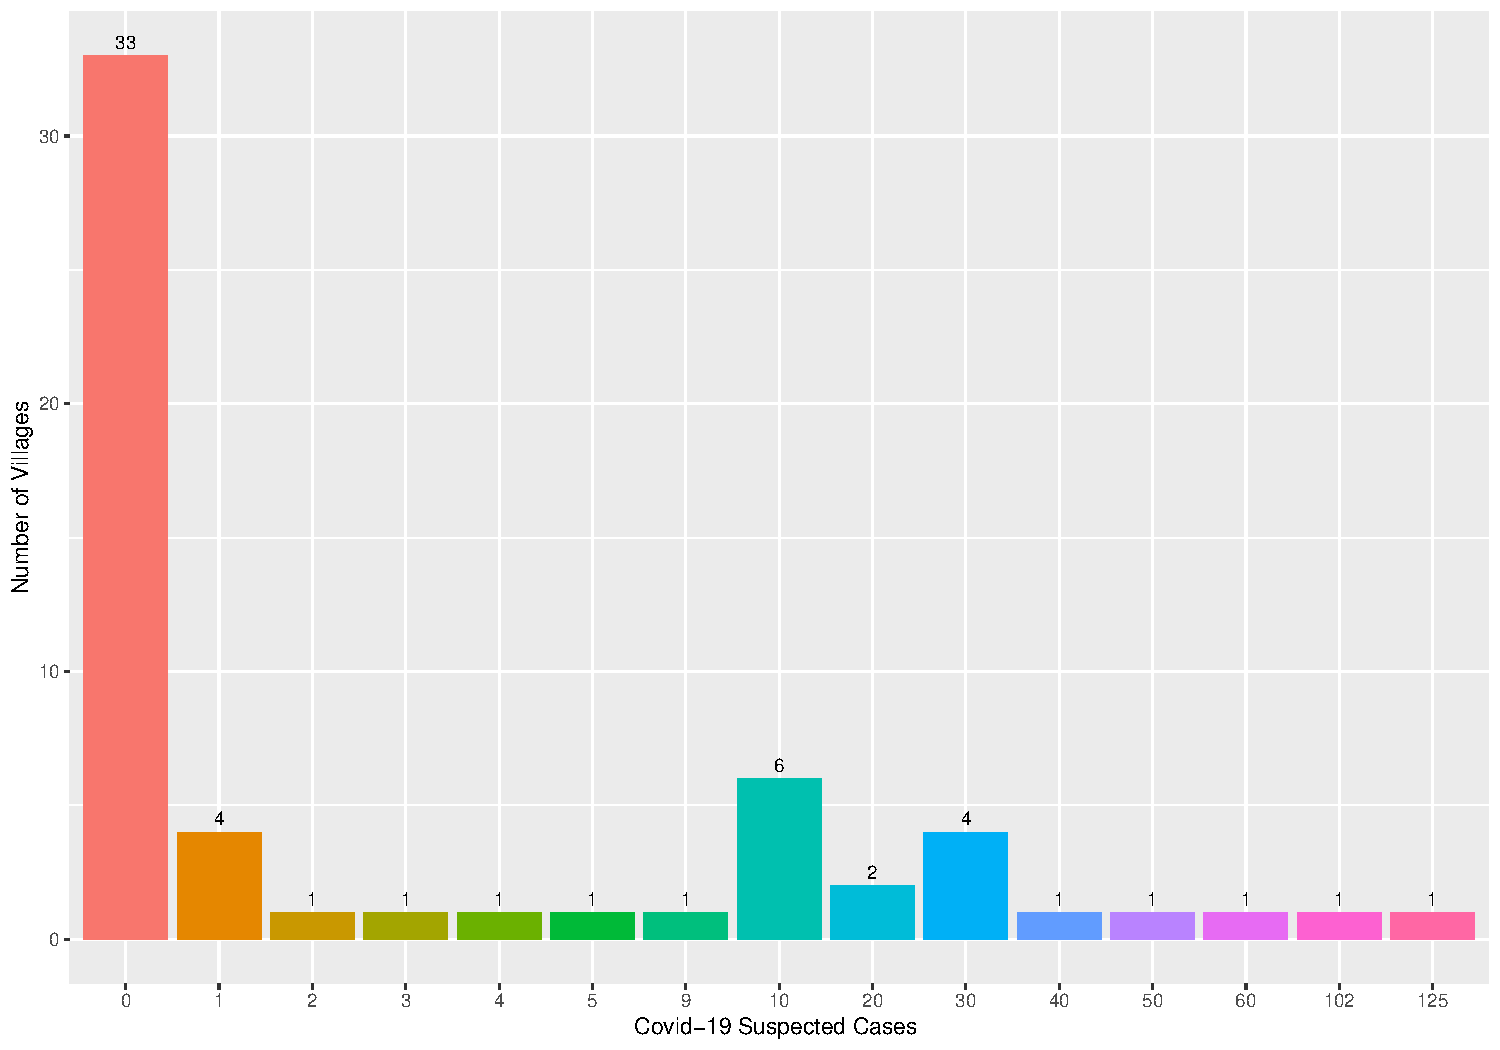
\includegraphics[width=1\linewidth]{example_plots_files/figure-beamer/unnamed-chunk-8-1} \caption{Covid-19 suspected cases distribution}\label{fig:unnamed-chunk-8}
\end{figure}
\end{frame}

\begin{frame}{Covid-19 Confirmed Cases}
\protect\hypertarget{covid-19-confirmed-cases}{}
\begin{figure}
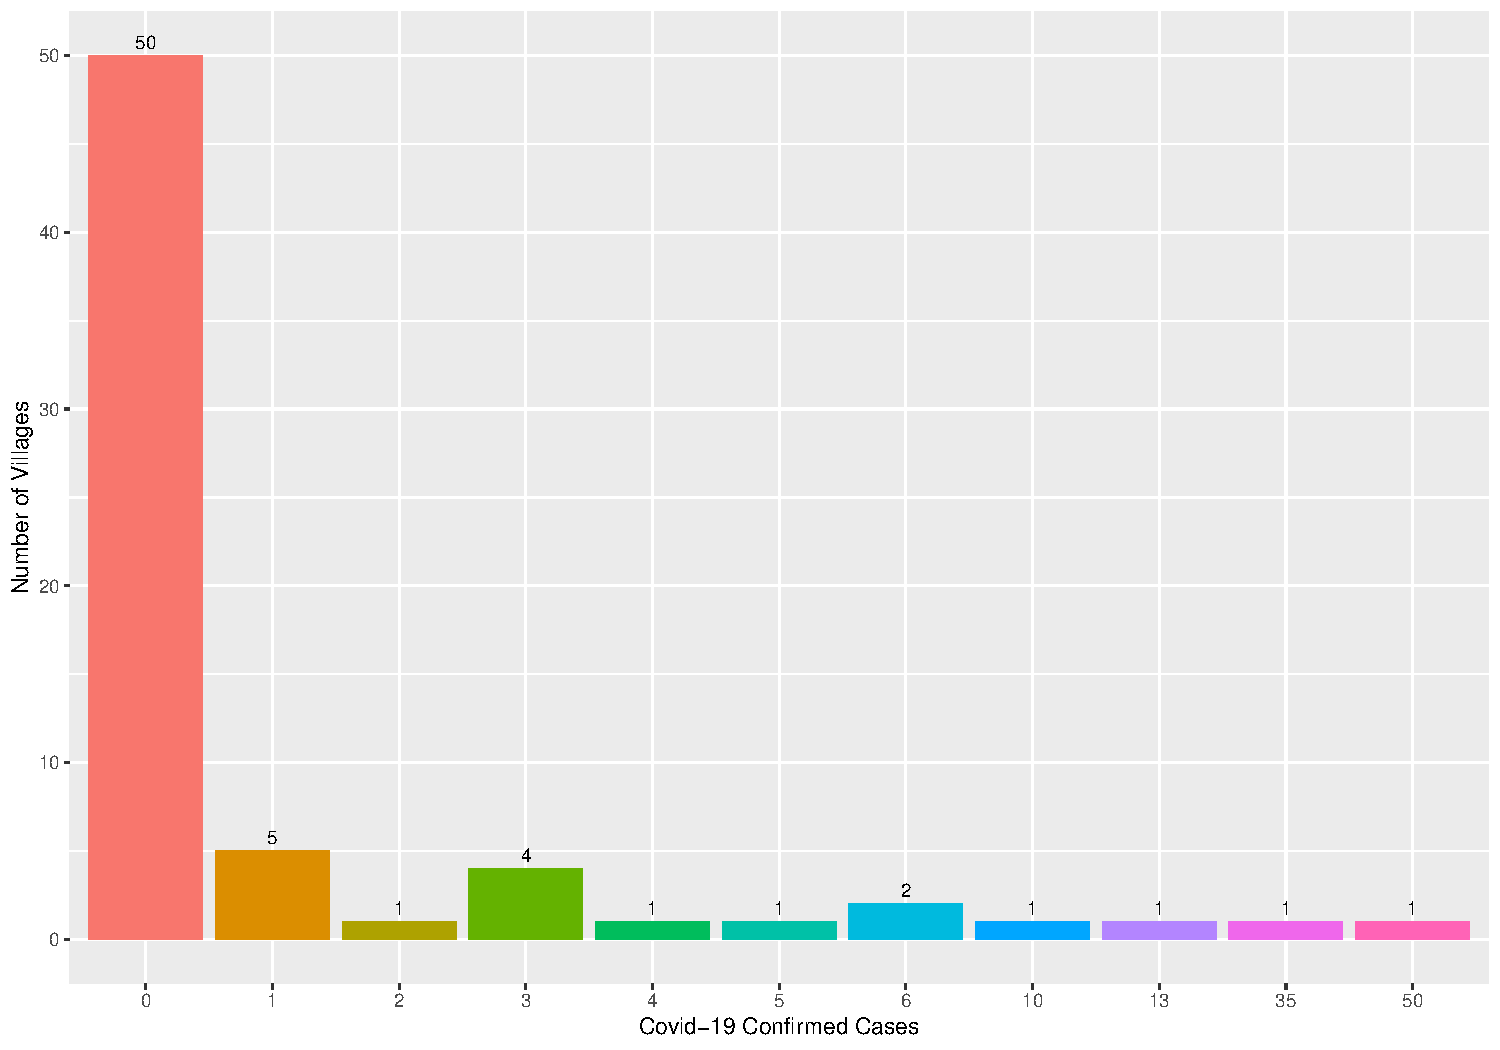
\includegraphics[width=1\linewidth]{example_plots_files/figure-beamer/unnamed-chunk-9-1} \caption{Covid-19 confirmed cases distribution}\label{fig:unnamed-chunk-9}
\end{figure}
\end{frame}

\begin{frame}{Covid-19 Cases}
\protect\hypertarget{covid-19-cases}{}
\begin{itemize}
\tightlist
\item
  majority of villages did not have suspected (33 out of 77) or
  confirmed cases (55out of 77)
\item
  wide variation of Covid-19 cases across different villages
\end{itemize}
\end{frame}

\begin{frame}{Treated Malnutrition Cases (overall sample)}
\protect\hypertarget{malnut}{}
\begin{figure}
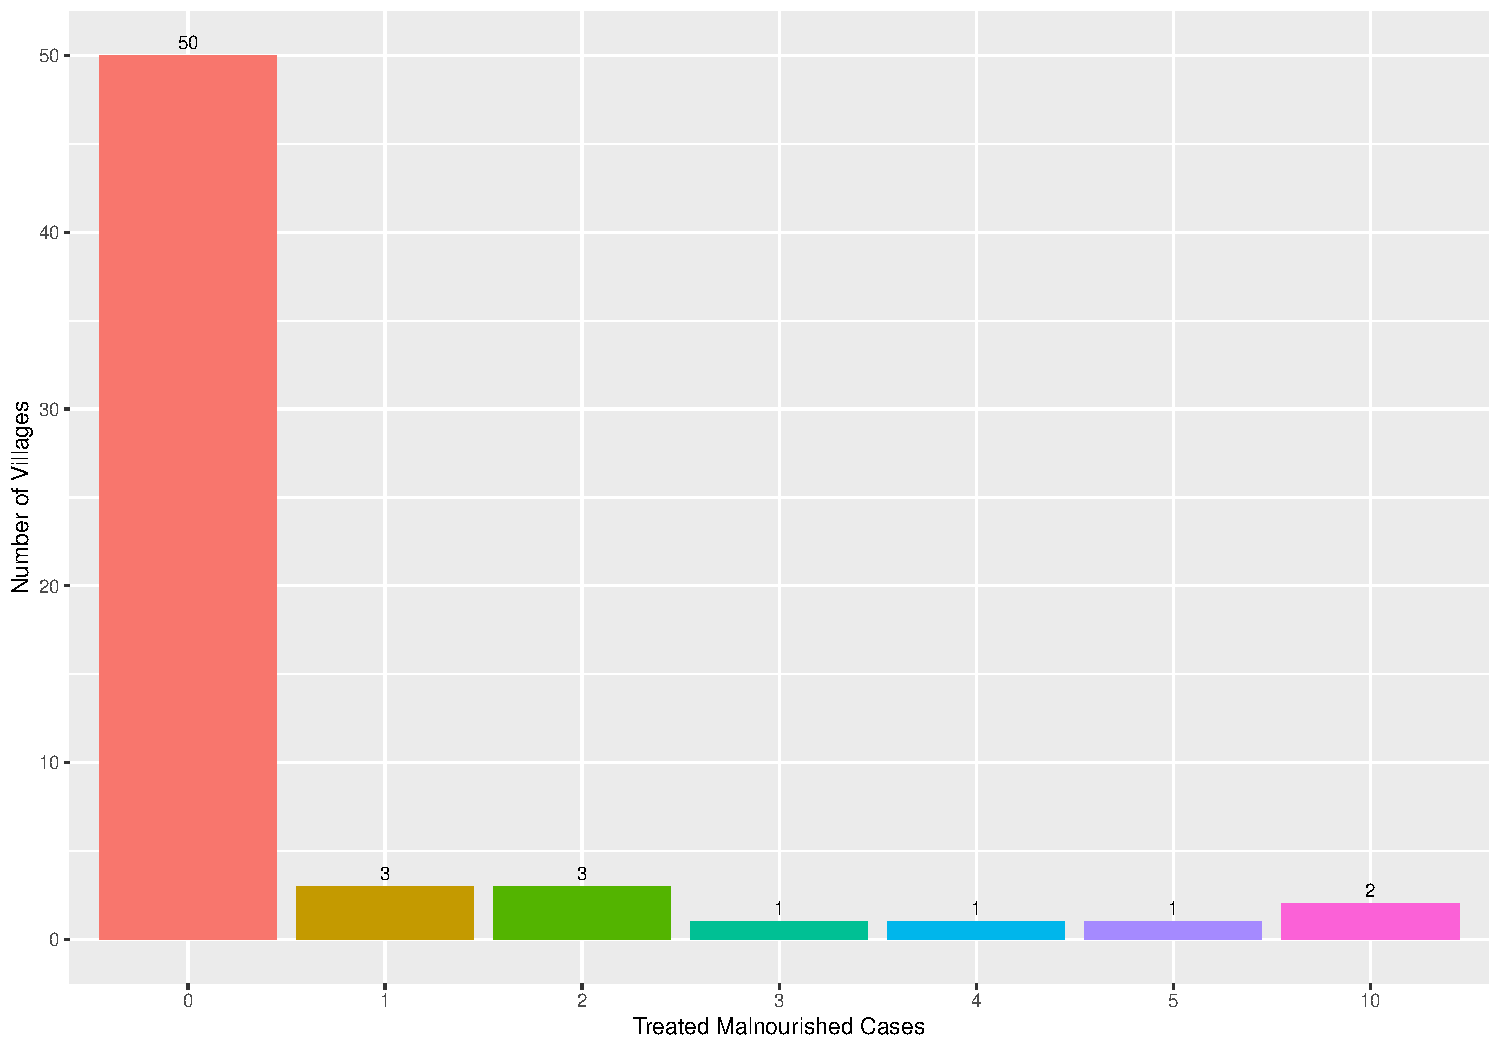
\includegraphics[width=1\linewidth]{example_plots_files/figure-beamer/unnamed-chunk-10-1} \caption{Treated malnourished cases distribution}\label{fig:unnamed-chunk-10}
\end{figure}
\end{frame}

\begin{frame}{Treated Malnutrition Cases (by sample type)}
\protect\hypertarget{treated-malnutrition-cases-by-sample-type}{}
\begin{figure}
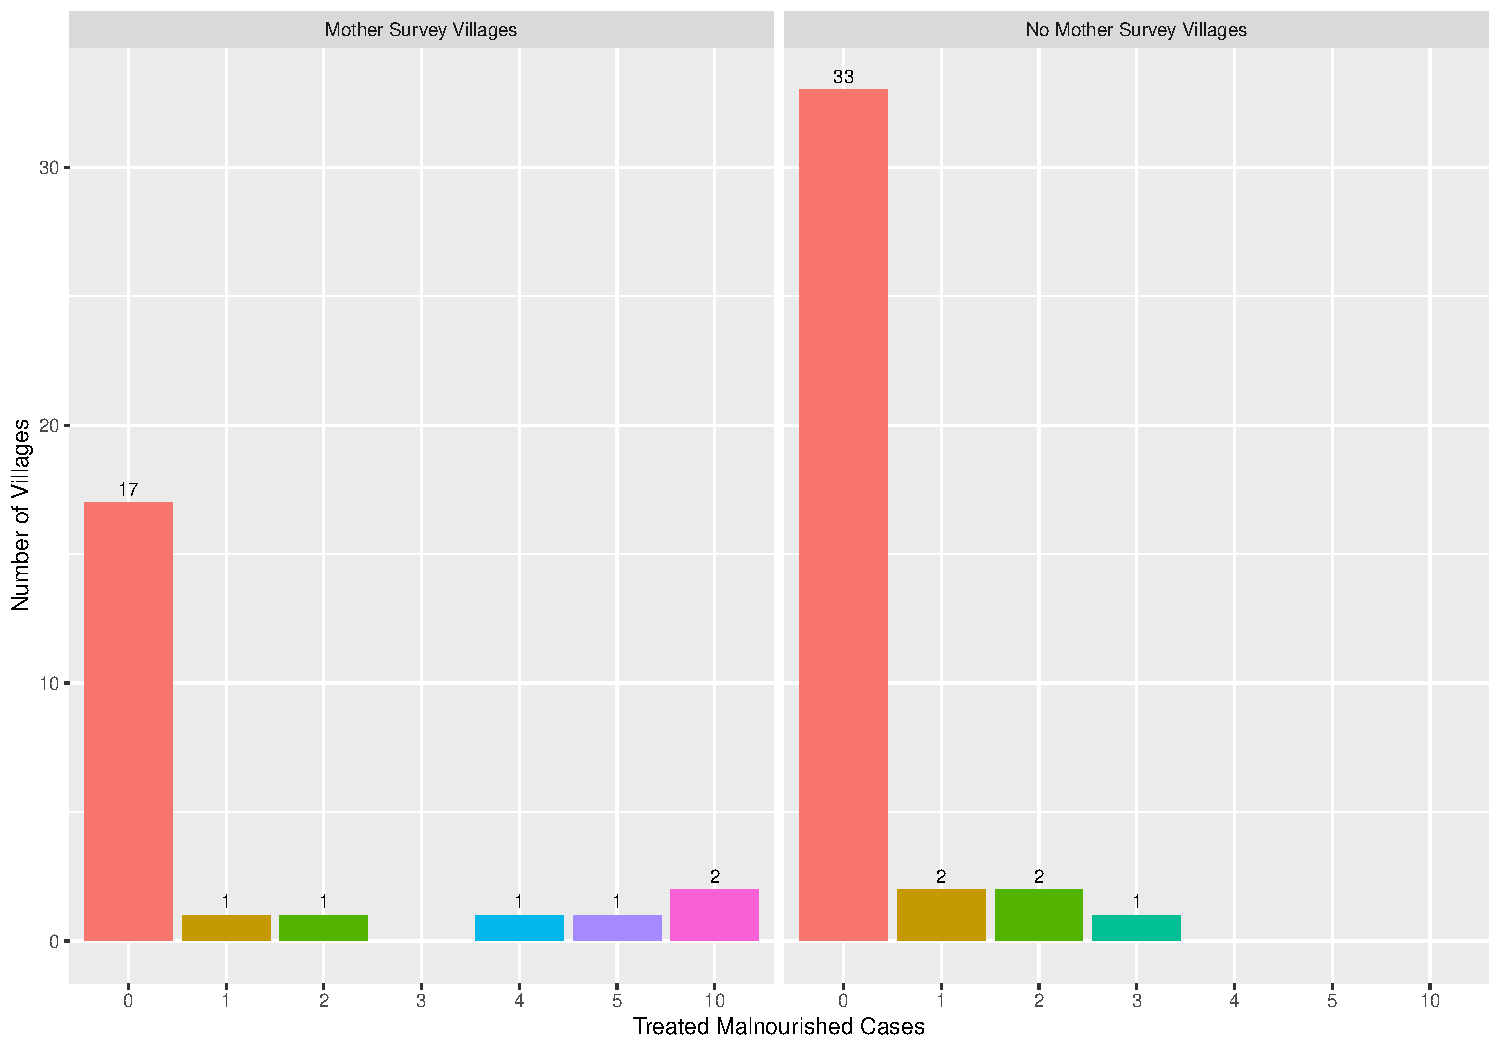
\includegraphics[width=1\linewidth]{example_plots_files/figure-beamer/unnamed-chunk-11-1} \caption{Treated malnourished cases distribution by sample type}\label{fig:unnamed-chunk-11}
\end{figure}
\end{frame}

\begin{frame}{Treated Malnutrition Cases}
\protect\hypertarget{treated-malnutrition-cases}{}
\begin{itemize}
\tightlist
\item
  majority of villages (55 out of 77) did not have treated malnourished
  cases.
\item
  but this did not tell about the number of undernourished cases from
  each surveyed village (as it was not covered in the survey
  questionnaire).
\end{itemize}
\end{frame}

\begin{frame}{Coping Strategies (overall sample)}
\protect\hypertarget{vthccsi}{}
\begin{figure}
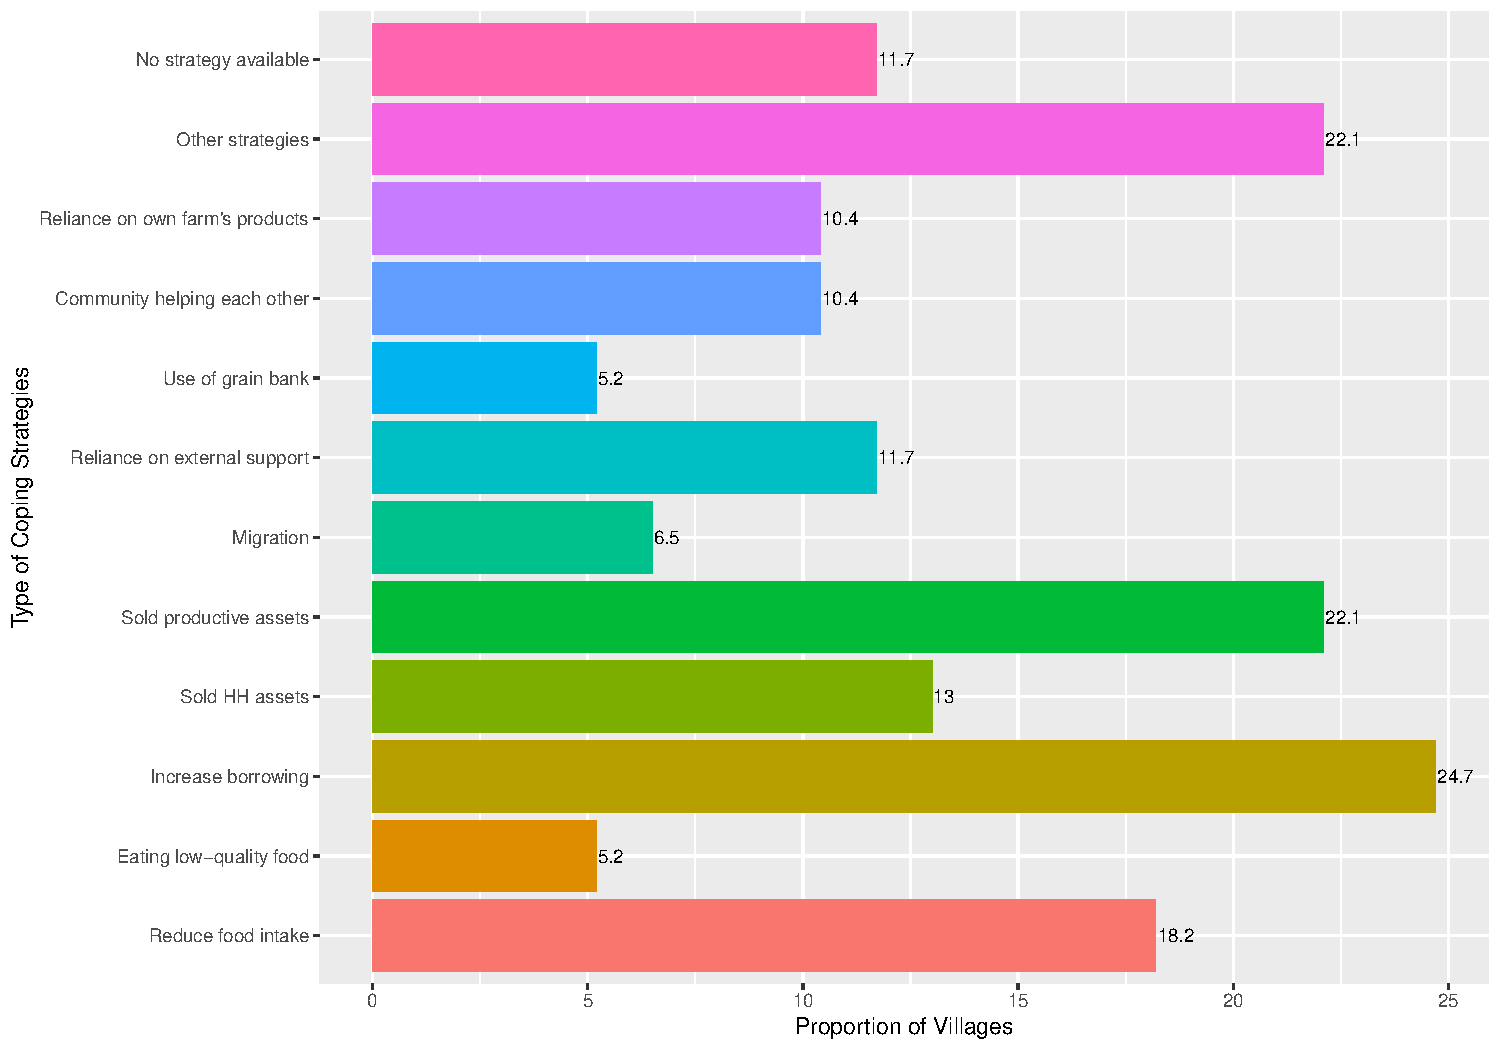
\includegraphics[width=1\linewidth]{example_plots_files/figure-beamer/unnamed-chunk-12-1} \caption{Common coping strategies distribution}\label{fig:unnamed-chunk-12}
\end{figure}
\end{frame}

\begin{frame}{Coping Strategies}
\protect\hypertarget{coping-strategies}{}
\begin{itemize}
\tightlist
\item
  Increasing borrowing (24.7\%), selling productive assets (22.1\%), and
  reduced food intakes (18.2\%) were the most reported categories\\
\item
  one-fifth of the sample reported other strategies (22.1\%), and most
  of their answers were that they had not experienced the condition
  which required applying the coping mechanism
\end{itemize}
\end{frame}

\begin{frame}{Distance to Market (overall sample)}
\protect\hypertarget{markets}{}
\begin{figure}
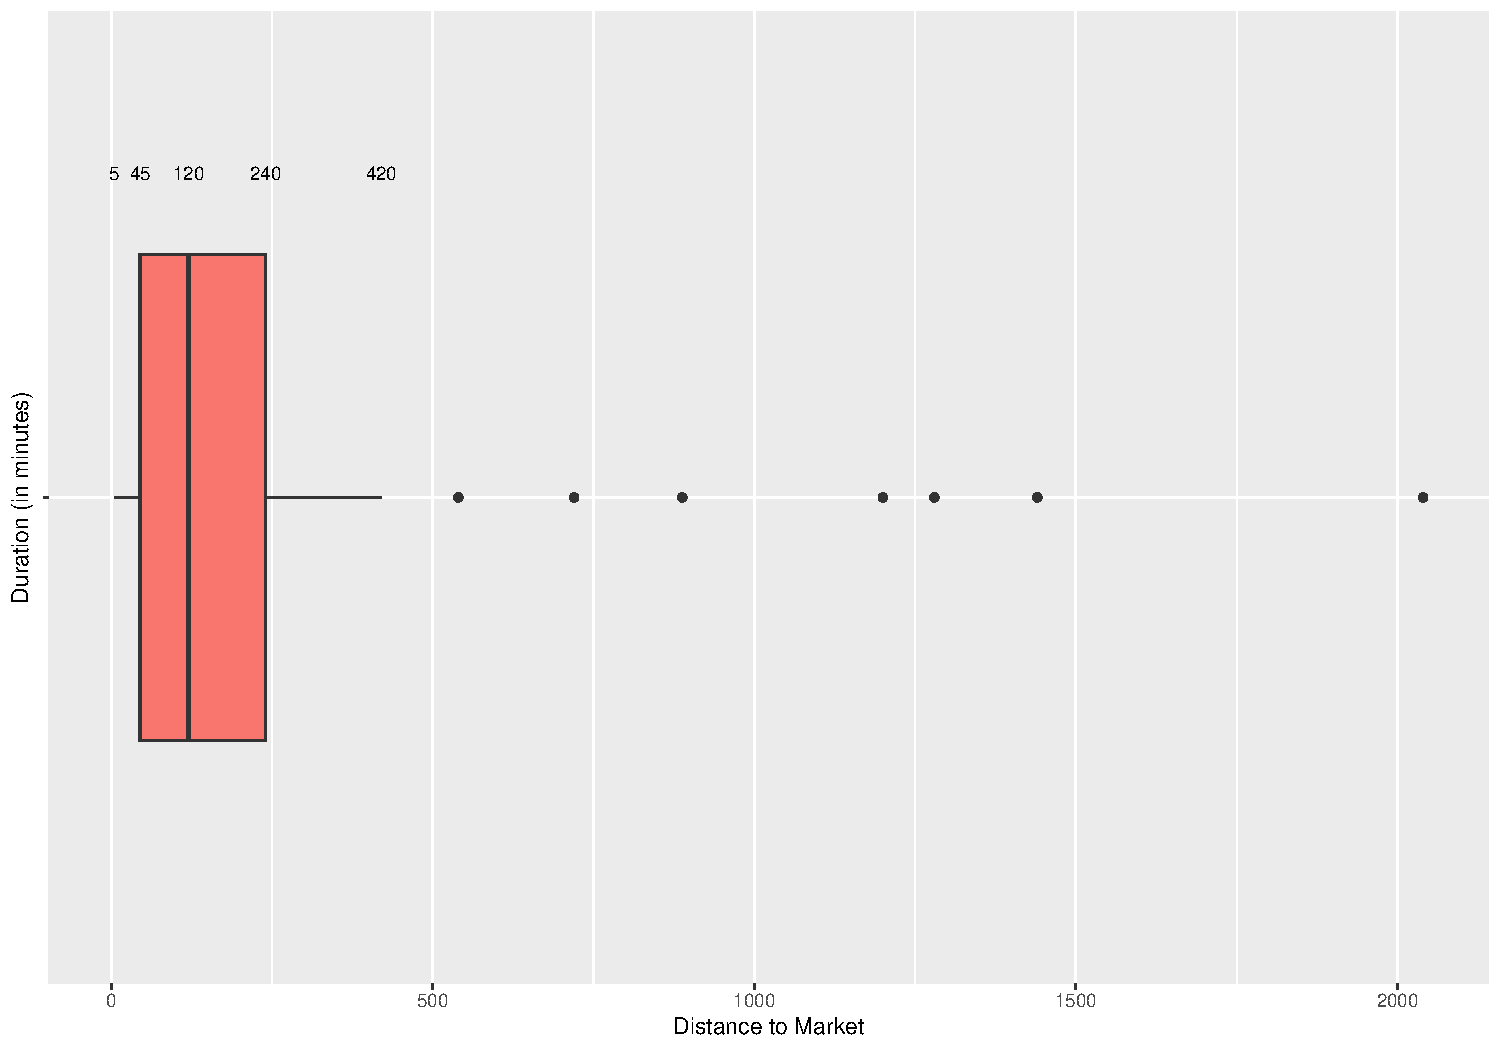
\includegraphics[width=1\linewidth]{example_plots_files/figure-beamer/unnamed-chunk-13-1} \caption{Walking distance to market distribution}\label{fig:unnamed-chunk-13}
\end{figure}
\end{frame}

\begin{frame}{Distance to Market (by sample type)}
\protect\hypertarget{distance-to-market-by-sample-type}{}
\begin{figure}
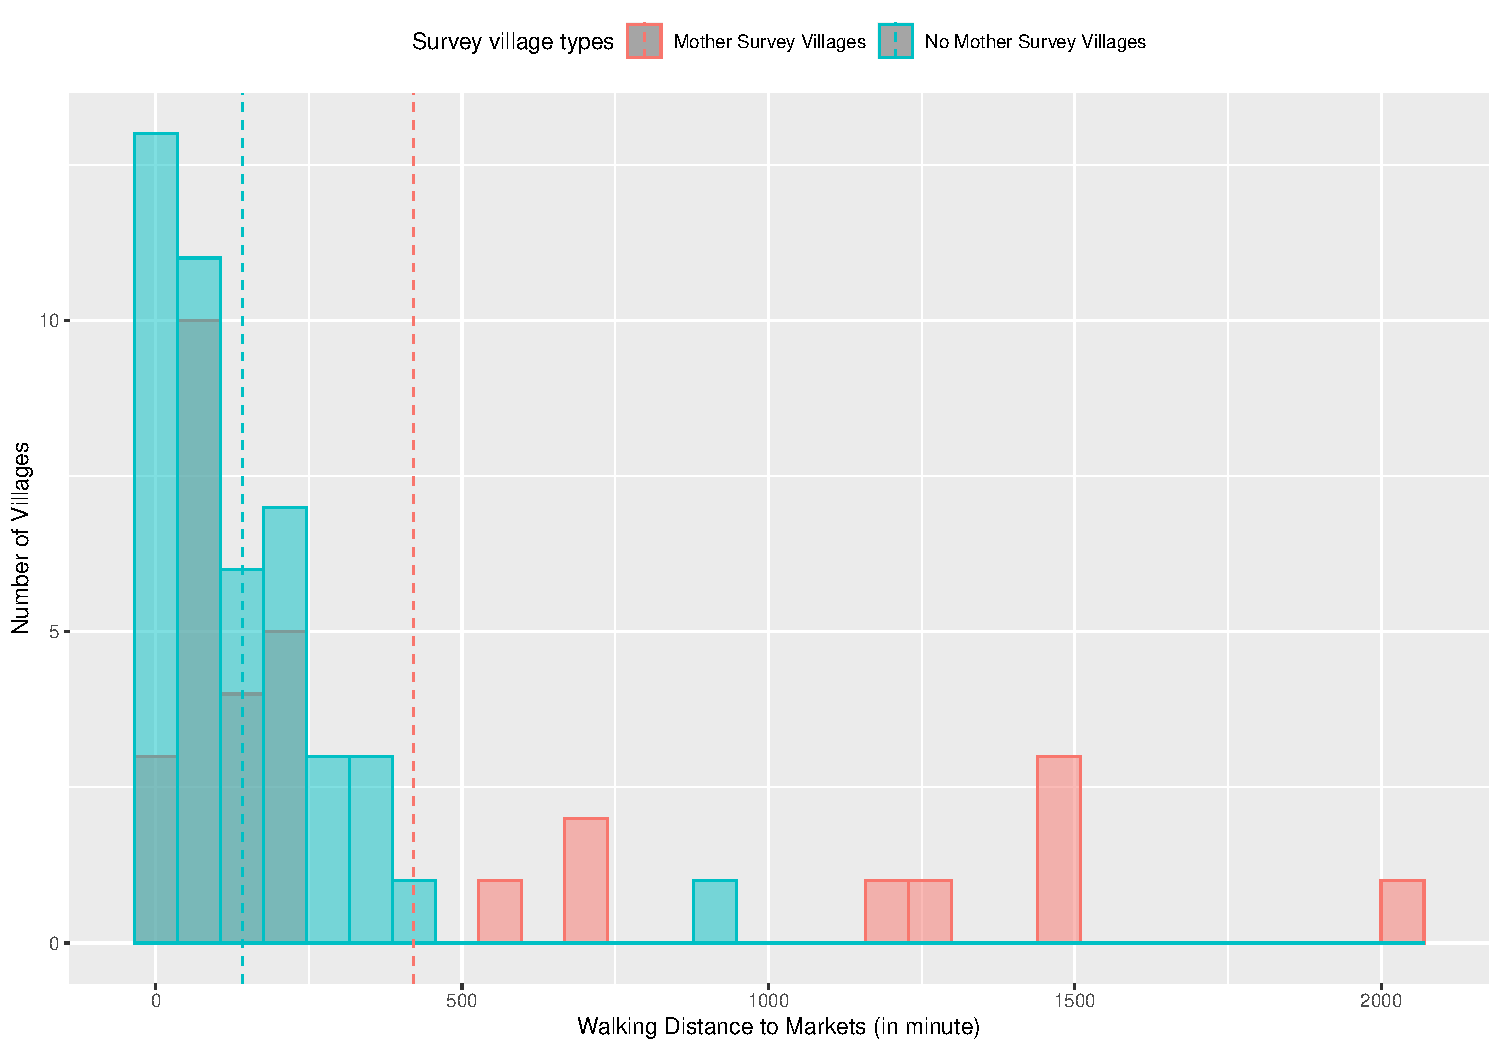
\includegraphics[width=1\linewidth]{example_plots_files/figure-beamer/unnamed-chunk-14-1} \caption{Walking distance to market distribution by sample type}\label{fig:unnamed-chunk-14}
\end{figure}
\end{frame}

\begin{frame}{Distance to Market}
\protect\hypertarget{distance-to-market}{}
\begin{itemize}
\tightlist
\item
  more villages required walking more than 2 hours (120 minutes)\\
\item
  travel distances widely varied across villages, and outlier villages
  were identified (with over 12 hours of walking distance)\\
\item
  mother survey villages required more travel time to access the market
  (median value - 2 hours), while the VTHC only surveyed village did
  1:30 hours
\end{itemize}
\end{frame}

\begin{frame}{Food commodity prices (overall sample)}
\protect\hypertarget{foodprices}{}
\begin{figure}
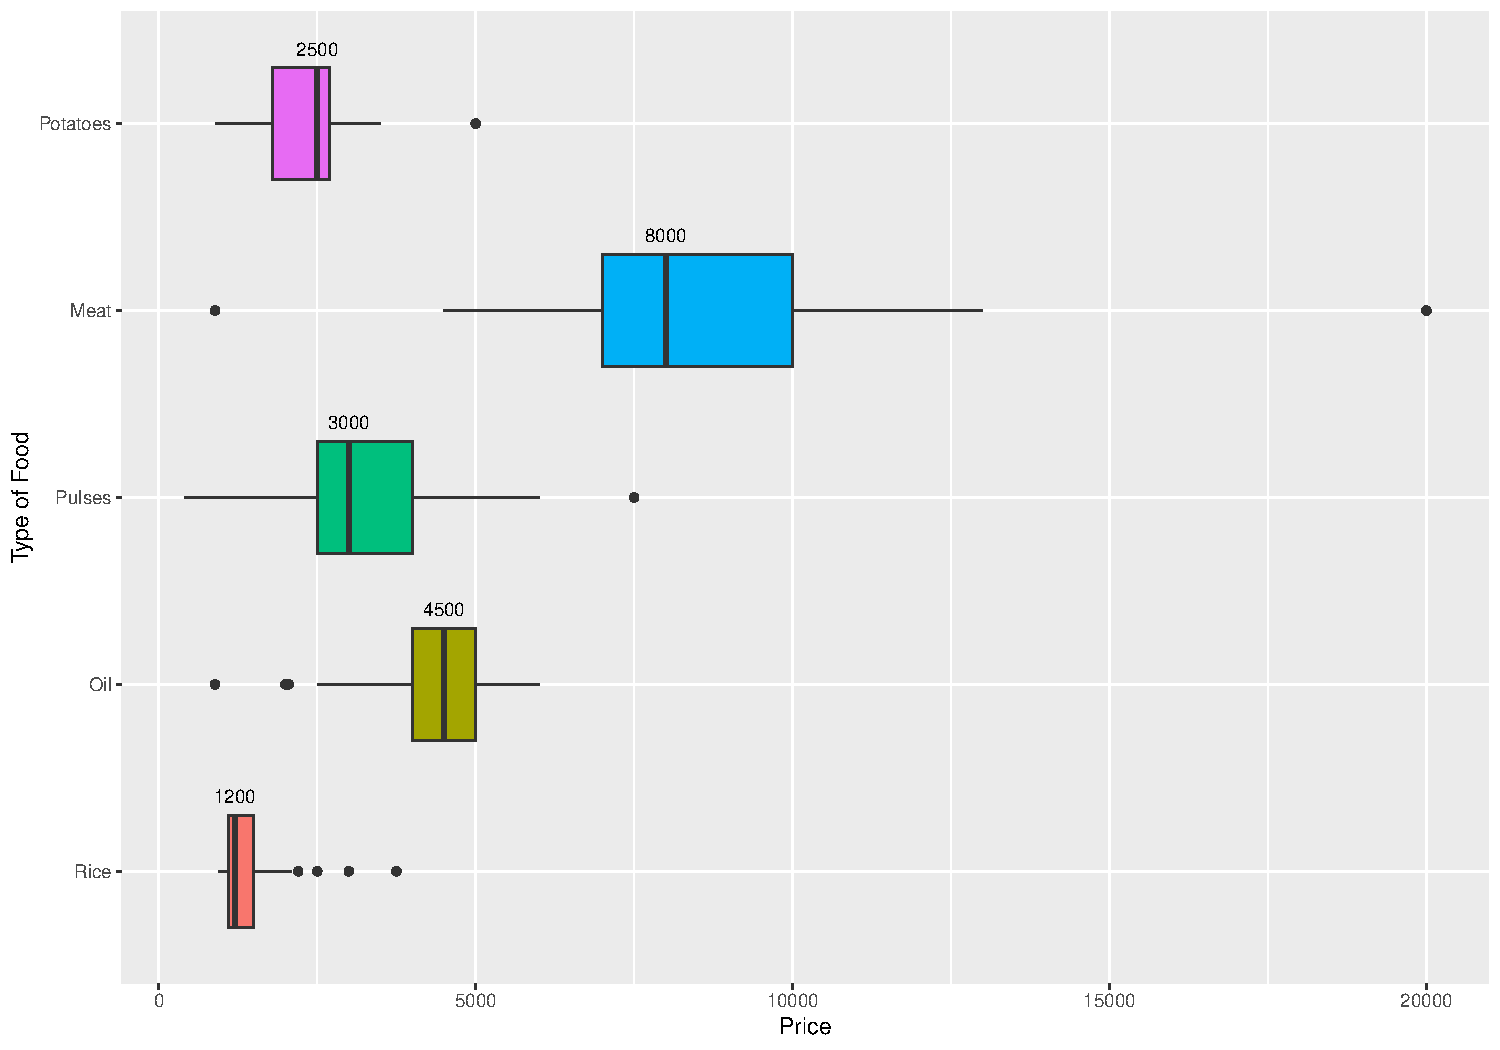
\includegraphics[width=1\linewidth]{example_plots_files/figure-beamer/unnamed-chunk-15-1} \caption{Food commodity price distribution}\label{fig:unnamed-chunk-15}
\end{figure}
\end{frame}

\begin{frame}{Food commodity prices (by sample type)}
\protect\hypertarget{food-commodity-prices-by-sample-type}{}
\begin{figure}
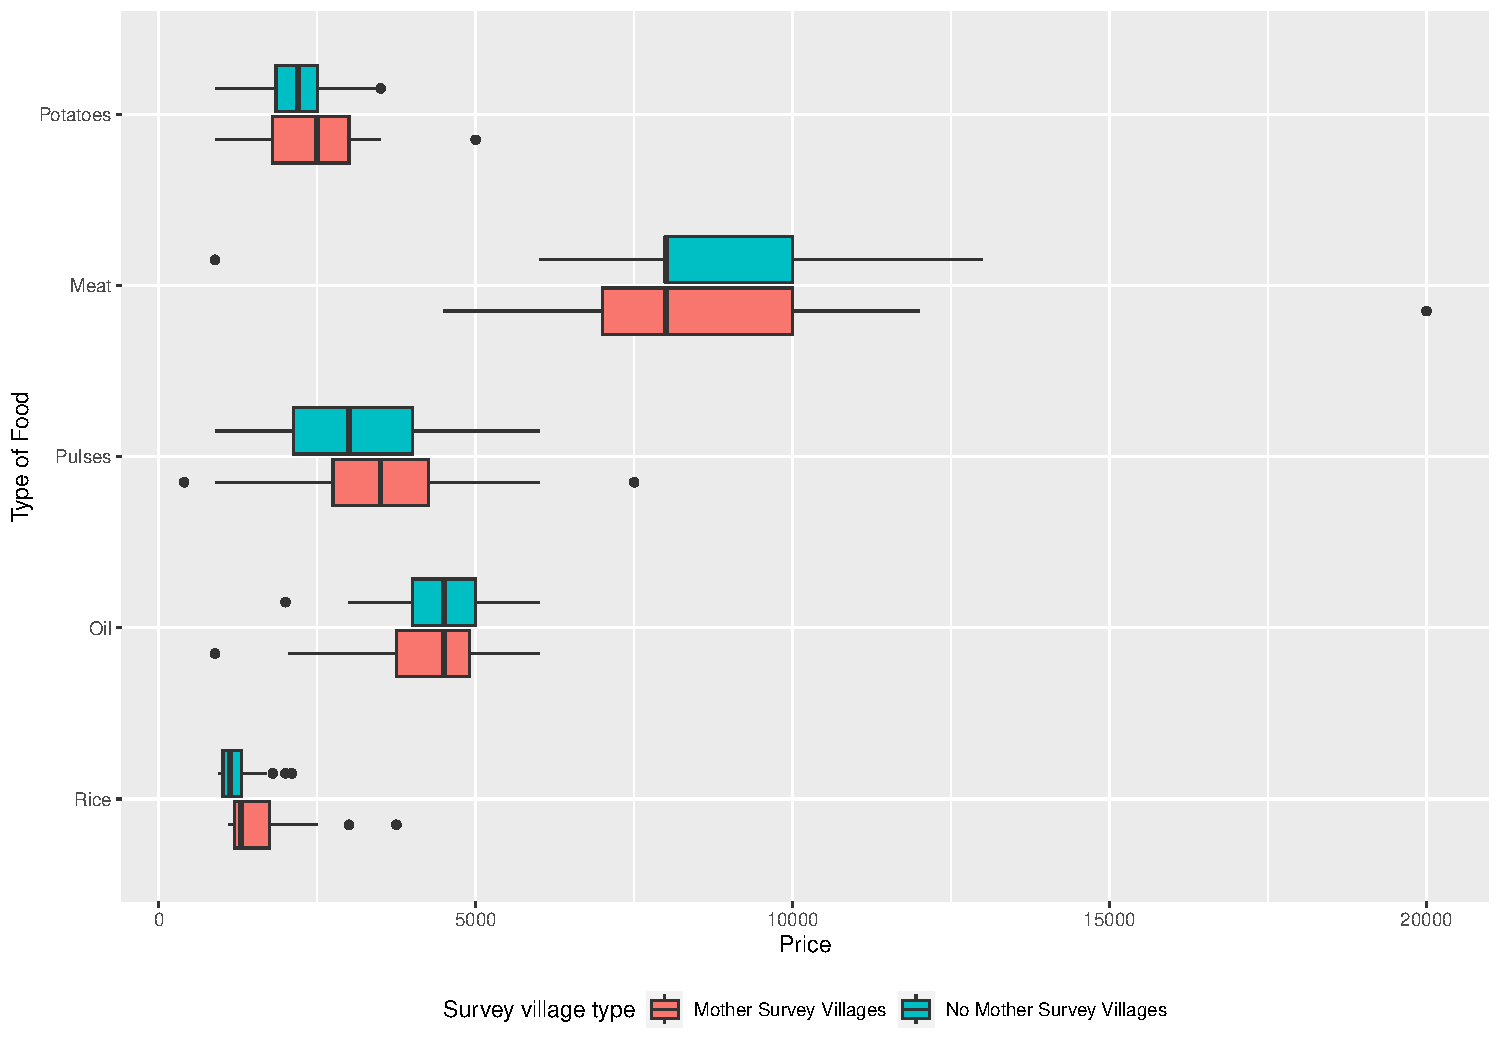
\includegraphics[width=1\linewidth]{example_plots_files/figure-beamer/unnamed-chunk-16-1} \caption{Food commodity price distribution by sample type}\label{fig:unnamed-chunk-16}
\end{figure}
\end{frame}

\begin{frame}{Food commodity prices}
\protect\hypertarget{food-commodity-prices}{}
\begin{itemize}
\tightlist
\item
  wide price variations were detected in meat and pulses food groups\\
\item
  although the price had minor price variation compared to the above
  food groups, more outlier prices were seen, and more villages had
  higher prices than their median price value\\
\item
  mother survey villages had a higher price for rice and potatoes but a
  lower oil price (statistically significant)
\end{itemize}
\end{frame}

\begin{frame}{Telecom Availability (overall sample) \{telecon\}}
\protect\hypertarget{telecom-availability-overall-sample-telecon}{}
\begin{figure}
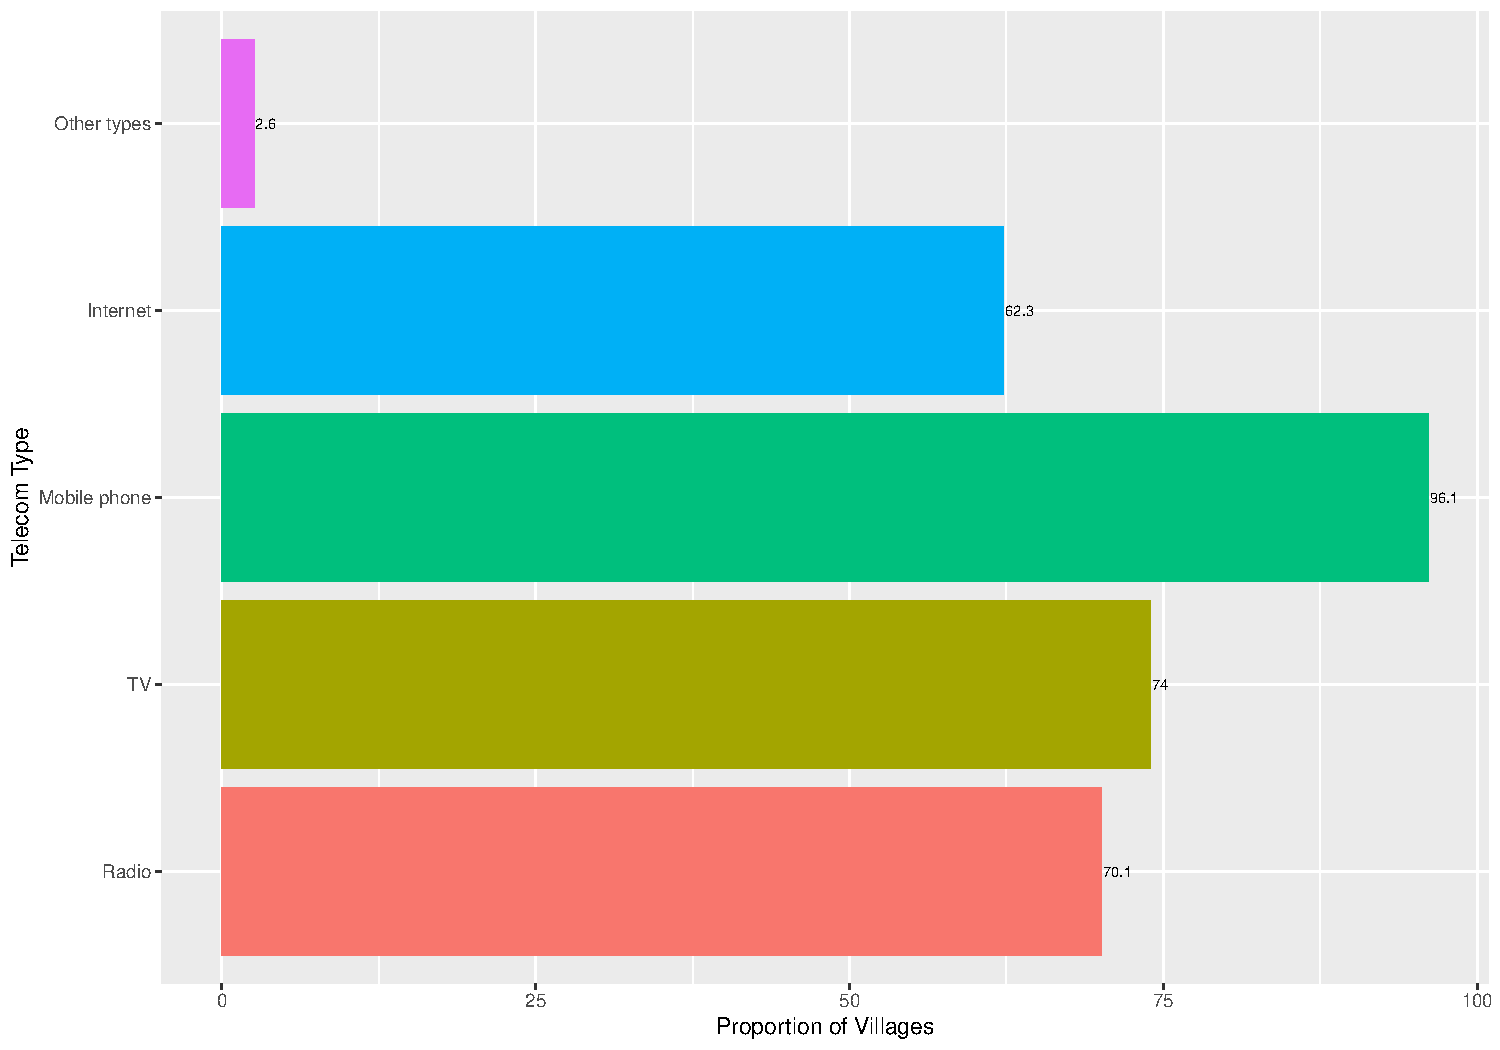
\includegraphics[width=1\linewidth]{example_plots_files/figure-beamer/unnamed-chunk-17-1} \caption{Telecom availability distribution}\label{fig:unnamed-chunk-17}
\end{figure}
\end{frame}

\begin{frame}{Telecom Availability (by sample type)}
\protect\hypertarget{telecom-availability-by-sample-type}{}
\begin{figure}
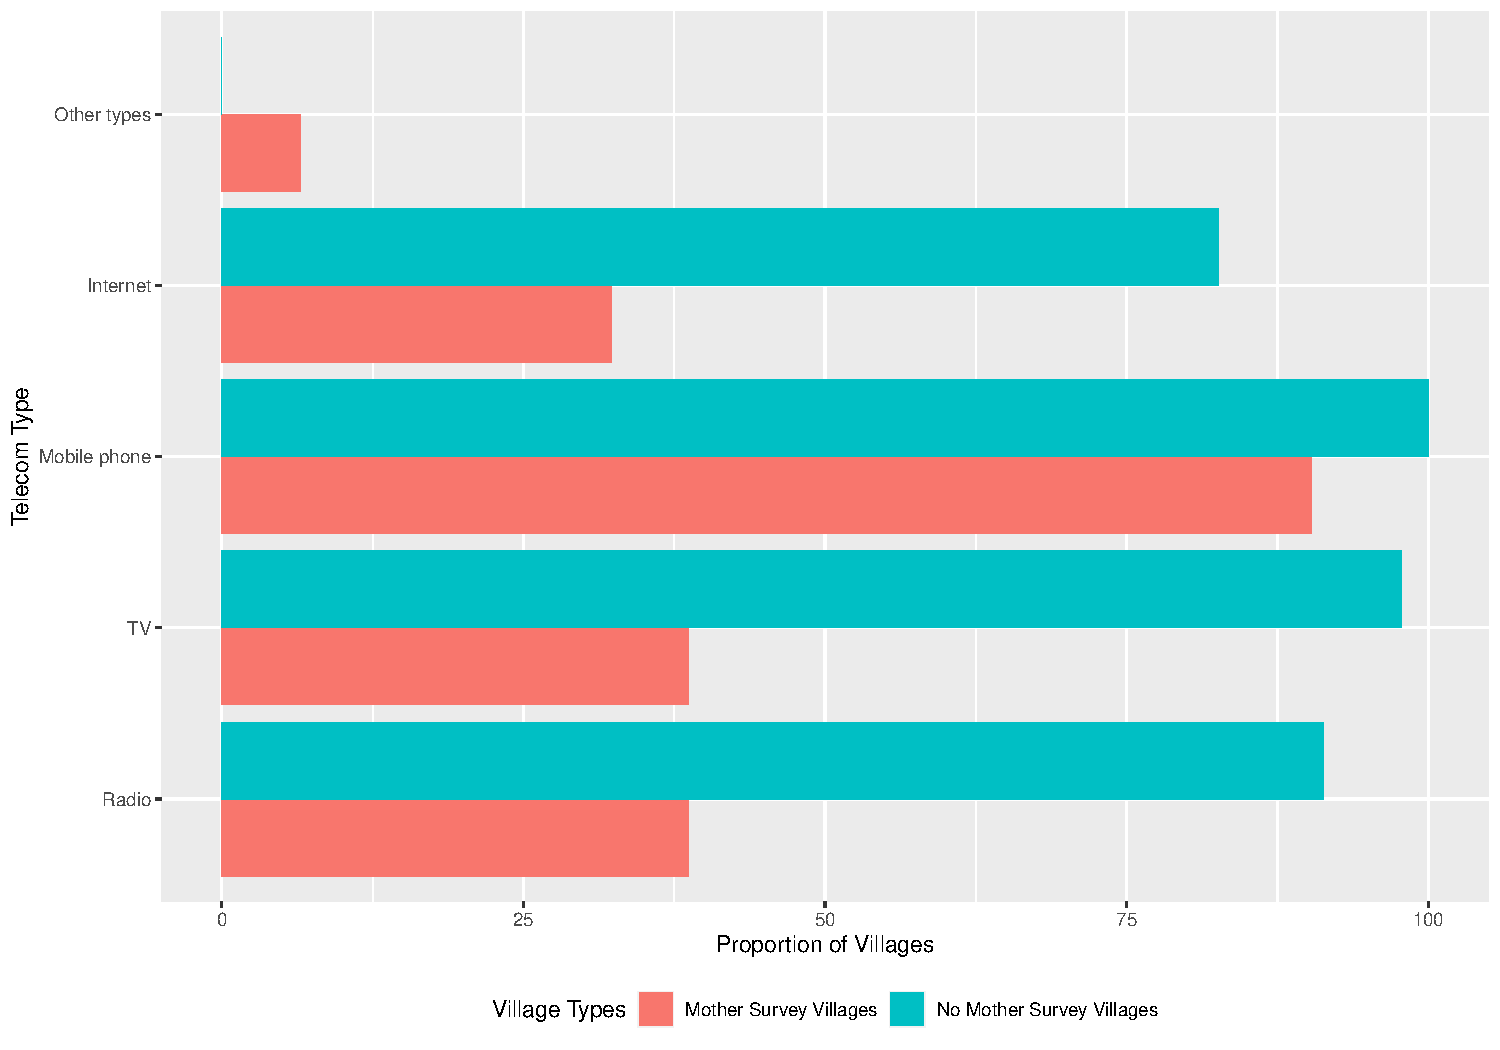
\includegraphics[width=1\linewidth]{example_plots_files/figure-beamer/unnamed-chunk-18-1} \caption{Telecom availability distribution by sample type}\label{fig:unnamed-chunk-18}
\end{figure}
\end{frame}

\begin{frame}{Telecom Availability}
\protect\hypertarget{telecom-availability}{}
\begin{itemize}
\tightlist
\item
  almost all surveyed villages (96.1\%) had mobile phone access, but
  just over two-thirds of the villages got access to the internet
\item
  majority of villages had the better coverage of radio and TV (over
  70\%) {[}means access to TV and radio, not all HHs from each village
  had radio or TV)
\item
  only VTHC survey villages had the better condition in telecom
  accessibility
\end{itemize}
\end{frame}

\end{document}
